
%(BEGIN_QUESTION)
% Copyright 2006, Tony R. Kuphaldt, released under the Creative Commons Attribution License (v 1.0)
% This means you may do almost anything with this work of mine, so long as you give me proper credit

An important numerical constant related to the von K\'arm\'an effect is the {\it Strouhal number}.  Explain what this number means, and why its constant (unchanging) value is important to flow-measuring instruments based on the von K\'arm\'an effect.

\underbar{file i00492}
%(END_QUESTION)





%(BEGIN_ANSWER)

The Strouhal number (approximately equal to 0.17) is the ratio of a blunt object's width to the distance between successive fluid vortices spilling off of the side of that object.

$$\includegraphics[width=15.5cm]{i00492x01.eps}$$

$${d \over \lambda} = 0.17$$

\vskip 10pt

In essence, the Strouhal number tells us that the {\it wavelength} ($\lambda$) of vortex ``waves'' is always constant given a bluff body of constant width.  Therefore, the frequency of these waves is directly proportional to the velocity of the fluid (and thus the volumetric flow rate in a pipe of constant cross-sectional area).

\vskip 10pt

It should also be noted that wavelength ($\lambda$), wave velocity ($v$), and wave frequency ($f$) are related to each other by the following equation:

$$v = f \lambda$$

Dimensional analysis helps prove this is true:

$$\left[\hbox{meters} \over \hbox{second}\right] = \left[\hbox{cycles} \over \hbox{second}\right] \left[\hbox{meters} \over \hbox{cycle}\right]$$

My choice to use ``meters'' here is arbitrary.  The relationship is true regardless of length unit (feet, inches, centimeters, miles, cubits, whatever!).

%(END_ANSWER)





%(BEGIN_NOTES)


%INDEX% Physics, dynamic fluids: Strouhal number
%INDEX% Physics, dynamic fluids: von Karman effect

%(END_NOTES)


